\documentclass[twocolumn,11pt]{article}

\usepackage[margin=1in]{geometry}
\usepackage{caption}
\usepackage{graphicx}

\title{Journey: A Study in Unhelpful Titles (TODO: should we get a new title?)}
\author{Mark Mansi, Suhas Pai, Hasnain Ali Pirzada\\\texttt{\{markm, hp, spai\}@cs.wisc.edu}}
\date{}

\begin{document}

\maketitle

\section{Introduction}

Recent advances in memory technologies are making it possible for machines with
large amounts of memory to become commonplace. Many current systems already
have dozens or hundreds of gigabytes of memory. These technology advances can
enable systems with terabytes of memory in the not very distant future. For
example, non-volatile memory technologies, which have denser physical
structures than traditional DRAM are making such large memories available and
more accessible \cite{xpoint}.

Much research is currently being done to study how non-volatile and large
memory systems would change system design. HP has been working on a system
which it calls ``The Machine'', in which hundreds of cores have access to a
multi-petabyte shared memory pool \cite{hp_machine}. Intel and
Micron have announced their 3D Xpoint non-volatile memory technology, making
dense, fast, persistent memory comercially available \cite{xpoint}.

However, studies of large-memory systems are often forced to use simulation or
emulation to evaluate solutions because most researchers do not have access to
these sorts of systems for experimentation \cite{quartz}. This often
forces researchers to simplify models, incurring inaccuracy, or to use smaller
benchmarks, which are less realistic. We note that there was a similar problem
when large storage systems first became available \cite{david, exalt}.

Currently, there are few good tools available to systems researchers for
understanding how systems interact with large memories. We see the need for a
general lightweight technique or tool for studying and designing operating
systems capable of handling large memory while using systems currently
available to researchers.  An important first step towards building such a tool
is to identify bottlenecks in managing large memories that make a tool
difficult to develop. 

In particular, we look at the case of a single process using a large amount of
memory in Linux. We run experiments to identify the costs of
\texttt{vm\_area\_struct}, a common bookkeeping data structure in the Linux
kernel, along with the memory and processing overheads of swapping. From these
data, we extrapolate to systems running with more memory with an eye on
implications for studying large systems. While these experiments are not
comprehensive, we believe they can offer insights that are useful both for
building a research tool and for building systems.


\section{Background}

In our methodology, we run several experiments to measure the scalability of
the Linux memory management system. Each experiment is designed to probe a
different aspect of the system. This section gives some background knowledge
necessary to understanding the experiments.

\subsection{Virtual Memory Areas}

A process may use the \texttt{mmap} system call to request that the kernel
allocate part of its virtual address space. Accesses to memory addresses
outside of allocated regions result in a segmentation fault. This makes memory
corruption errors easier to find and debug, and increases security from memory
corruption attacks.

The Linux kernel keeps track of which portions of a process's address space
have been allocated using the \texttt{vm\_area\_struct}. Because processes may
map a number of regions, including shared objects, stack, heap, text, and
anonymous regions, the scalability of this structure is critical to Linux's
performance.

When a process maps a region, a \texttt{vm\_area\_struct} is created, but no
memory is allocated. When a process first touches a page, a page fault occurs
and the processor traps into a page fault handler, which can allocate memory
and set up a page table entry. This is called demand paging.

For demand paging to work efficiently, the correct \texttt{vm\_area\_struct}
needs to be efficient to find. Linux caches the most recently used region and
organizes all regions into a balanced binary tree for fast lookup.  Moreover,
adjacent regions with similar permissions and properties are merged in an
effort to keep bookkeeping costs low.

(TODO: explain struct page?)

We measure the memory overhead and latency of the Linux Memory Management
system's use of \texttt{vm\_area\_struct}, which represents a region of a
process's virtual address space.  
We do not measure the overhead of \texttt{struct page} because it is known that
there is one struct for each physical page. We do not measure the overhead of
page tables because this can be calculated from the size of the virtual memory
space used by the process.  When a program makes a memory management system
calls such as \texttt{mmap}, \texttt{mremap}, \texttt{munmap},
\texttt{mprotect}, \texttt{mlock}, or \texttt{madvise}, the kernel is creating,
changing, or removing \texttt{vm\_area\_struct}s; thus, measuring the
scalability of Linux memory management requires measuring the overhead of these
structs.

\subsection{Swapping}

Under memory pressure, the kernel may choose to write some pages of memory to
disk and then free those pages for use. Memory mapped files are written back to
their backing files, but anonymous memory is written to portion of the disk
called swap space. We focus on anonymous memory in our experiments.

Before swapping a page out to disk, the kernel must reserve a slot for the page
in the swap space, unmap it from the process's address space, and record which
swap slot corresponds to the page.

On Linux, the system may have multiple swap spaces in the form of a swap disk
partition or of swapfiles on a filesystem. Both have a similar format on disk,
in which the space is broken into a number of swap slots large enough for one
page. For each of these swap spaces, the kernel keeps a swap map, which records
the usage of each swap slot so that it can find and allocate them quickly.

Unmapping a page from a process's address space involves simply marking its page
table entry ``Not Present''. Rather than using a separate data structure, Linux
uses the unused page table entry to record information about which swap space
and slot is used to swap out the page.

When a system uses huge pages and is low on memory, they are not swapped as is.
The huge pages are broken down to their component small pages, which are then
swapped to disk. This is done to prevent complication of the swapping logic in
the kernel, but results in additional overheads. \cite{corbet_transparent}

\subsection{Page Frame Reclamation}

To determine which pages to swap out, Linux uses the Page Frame Reclamation
subsystem. Choosing which pages to swap out is important because if the system
swaps out pages that are about to be used, thrashing may be induced, in which
the system wastes lots of time swapping out a page just swap it back in.

The Linux Page Frame Reclamation Algorithm (PFRA) attempts to approximate LRU
order. It uses a clock-like algorithm, in which a list of pages is scanned
twice. Roughly speaking, if a page is not used between scans, then it is a
condidate for reclamation.

The PFRA runs primarily as a kernel thread called kswapd. kswapd runs at regular
intervals and sleeps in between. Also, it may be invoked if the system detects
that memory has gone below a threshold. kswapd will continue to run until enough
pages are freed to bring the free memory pool above some threashold. Then,
kswapd goes back to sleep.  One concern with large memory systems is that kswapd
may expend significant CPU time scanning through hundreds of thousands of pages.

\section{Methodology}

We conduct a series of experiments to measure the scalability of various parts
of the Linux memory management system.  First, we measure the scalability of
Linux's \texttt{vm\_area\_struct}. Then, we measure the scalability of Linux's
swapping mechanisms.

\begin{figure}
\centering
\begin{tabular}{|l|p{5cm}|} \hline
OS & Ubuntu 16.04.2 \\ \hline
Kernel & Linux 4.4.0-70 \\ \hline
CPU & Intel Xeon E5645, 2.40 GHz, 6 cores/12 threads, 32kB L1-D, 32kB L1-I,
    256kB L2, 12MB L3 \\ \hline
Memory & 16GB, 1066MHz \\ \hline
Storage & 500GB HDD, 7200RPM \\
\hline
\end{tabular}
\caption{Specifications of our test machine.  \label{fig:specs}}
\end{figure}

The specifications of the machine we used to run our experiments are listed in
Figure \ref{fig:specs}. We disabled Intel SpeedStep and TurboBoost and ensure
that the processor frequency stays constant. All experiments are pinned to the
same core on our machine. 

We run several different microbenchmarks, each of which has a different memory
allocation pattern. These benchmarks are designed to stress the memory
management system in different ways, rather than simulate real workloads. 
Each run is executed in isolation, without any additional processes
running beyond services that start when the system is booted and a single ssh
session. We are careful to avoid opening extra ssh sessions, running screen or
tmux, or executing extra commands while a benchmark is running since these may
impact memory usage and, thus, our results.

We measured latency using the \texttt{rdtsc} instruction provided by x86\_64
processors, which gives high resolution cycle-level timestamps. We take a
timestamp before and after each memory management operation in the workload and
take the difference to get latency.

To measure memory usage, we use the procfs's reporting on current memory usage.
Where appropriate, we record the slab allocator's count of active
\texttt{vm\_area\_struct}s in the system. Measuring kernel memory usage and
associating memory usage with processes is difficult. Our methodology assumes
that our benchmarks are running in an otherwise idle system and should dominate
increases in memory usage.  We compute total memory usage by the rest of the
system as the total amount of memory less the amount of memory used by the
benchmark. We keep transparent huge pages on throughout our experiments, unless
otherwise specified.

To measure processor usage, we use the procfs's reporting on number of jiffies.
\texttt{/proc/stat} reports the number of jiffies of uptime the system has seen
overall, while \texttt{/proc/[pid]/stat} reports on the specified process.

\subsection{\texttt{vm\_area\_struct}}
\label{ss_vm_area_struct}

For each workload, we measure the latency and increase in memory usage due to
each operation in the benchmark. Notably, we do not touch the pages that we
allocate, avoiding both a page fault and the allocation of a back physical page
for the allocated virtual pages. This allows us to measure just the overhead of
memory management, as opposed to physical page allocation, swapping, page
faults, or other overheads.  Each workload contains $2^{20}$ memory management
operations.

Each benchmark was run 5 times and the results aggregated as described below. We
reboot the machine when switching to a different benchmark, but keep the machine
running continually during the runs of the same benchmark. 

Assume the memory usage of the rest of the system is $R$. We denote $R_i$ as the
$i$-th measurement of $R$ during a run ($i = 0, 1, ..., 2^{20}$). System memory
usage is known to jitter in Linux (TODO: cite). To adjust for this jitter, we
define $\Delta_i = R_i - R_0$. For each operation, we take the median value of
$\Delta_i$ across the 5 runs to reduce jitter further.  This is the value
graphed in the figures in the following section. $\Delta_i$ represents the
increase in memory usage due to memory management overheads caused by running
$i$ memory management operations.

The workloads we measure are

\begin{itemize} \item \textit{Control}. This workload is only run for the memory
overhead experiments. It simply prints the $\Delta_i$ for each $i$. It's graph
is a straight line with positive slope. This memory usage results from the
buffer containing stdout, where our readings are being printed. All of our
experiments have the same stdout overhead, so this benchmark serves a baseline
for comparison.

\item \textit{Continuous} (``cont'' for short). This workload allocates $2^{20}$
adjacent 16KB blocks.

\item \textit{Strided}. This workload allocates $2^{20}$ untouching 16KB regions
in order of increasing memory address.

\item \textit{Random}. This workload allocates randomly the pages in a
inside of a $2^{20}$ page region.

\item \textit{Fragmented} (``frag'' for short). This workload first allocates
    $2^{21}$ contiguous 4KB blocks. Then, it resizes every other block to 16KB.
        The resizing operation, rather than the initial allocation is measured.
\end{itemize}

\subsection{Swapping Memory Overhead}
\label{swapping_memory_overhead}

These experiments are designed to measure the minimum amount of memory needed
to using swapping.

A single process allocates 18GB of virtual memory space. It then proceeds to
write one byte of each 4KB page in the region, leading to the actual allocation
of physical memory. Notice that 18GB exceeds the 16GB of physical memory in the
test machine, causing Linux to start paging after physical memory is exhausted.
Also, notice that the Linux kernel will reserve some memory for its own
operation.

We run this experiment with both a continuous access pattern and a random access
pattern. The continuous access pattern simply touches adjacent pages in order of
increasing address. The random access pattern chooses a random address. Both
patterns touch the same number of addresses.

After each page of virtual memory is touched, the resident set size (RSS; the
amount of physical memory Linux has allocated to the process) is recorded.  The
values of RSS are stored in an mlocked array and written to a file after the
benchmark completes. This prevents the writing of the results from interacting
with paging in the kernel page cache. These RSS values are graphed in our
results section.

Moreover, we measure the latency of each memory store operation to see the
impact of swapping and virtual memory usage on memory access times.

We repeat this with 32GB of swap space and 128GB of swap space to see the
impact of swap space size on the amount of memory the kernel reserves for
itself, along with the impact on latency.

\subsection{kswapd}

These experiments are designed to measure the processing overhead of kswapd when
the system is under high memory pressure.

A single process allocates 18GB of virtual memory space and writes one byte of
each 4KB page in the region. The same two access patterns are tested as in the
previous set of experiments (continuous and random).

In all these experiments, the system is given 32GB of swap space total. We
repeat each experiment with hugepages enabled and disabled to see the impact of
the transparent hugepage system. The processor usage of kswapd and khugepaged is
recorded for each experiment and reported in the next section.

\section{Results}

\subsection{\texttt{vm\_area\_struct} Experiments}

\subsubsection{Time}

Figure \ref{fig:mmap_latency} shows for various microbenchmarks the time taken
per \texttt{mmap} operation as it varies with the total amount memory allocated
so far in the workload. 

It can be seen that for continuous \texttt{mmap}s the time is not only the
lowest but is also invariant with the total number of \texttt{mmap}s done so
far. There are two reasons for this. 

First, when a continuous \texttt{mmap} (with the same permissions) happens the
kernel memory allocator does not need to create a new \texttt{vm\_area\_struct},
instead it modifies the adjacent \texttt{vm\_area\_struct}s to account for the
newly allocated space. This avoids the need to use the slab allocator to create
a new struct. 

Second, for continuous \texttt{mmap} operations, the time taken is always the
lowest compared to other benchmarks.  This is because the kernel caches the most
recently used \texttt{vm\_area\_struct}, avoiding a red-black tree search. In
the continuous benchmark, this cached struct is always conveniently used.

For the other workloads, a search through the red-black tree is often needed on
most accesses. This operation takes $O(log n)$ time (where $n$ is the number of
virtual memory areas). The logarithmic behavior is visible in the plots for the
benchmarks in Figure \ref{fig:mmap_latency}.

The frag benchmark takes the most time of any benchmark. When a region of the
address space is being expanded, the kernel is forced to unmap it and map a new
area somewhere else.  This operation needs creation of a new memory area struct.
The kernel also must look through the red-black tree, though it never finds a
node which can be expanded to include the new mapping. Then, an insertion on the
tree is needed, possibly including rebalancing.

The strided workload is very similar to frag because it will also force the
kerenl to always create a new mapping and insert it into the tree after
traversing the tree first. It, however, does not need to delete an existing
mapping so it is faster than the frag benchmark. 

Finally, rand will also search through the red-black tree first but there is a
reasonably high probability that it will find an existing mapping adjacent to
the desired mapping which can be expanded, obviating the need to create a new
struct and insert it into red-black tree.

~\\ \textbf{Conclusions}

TODO?

\begin{figure}
    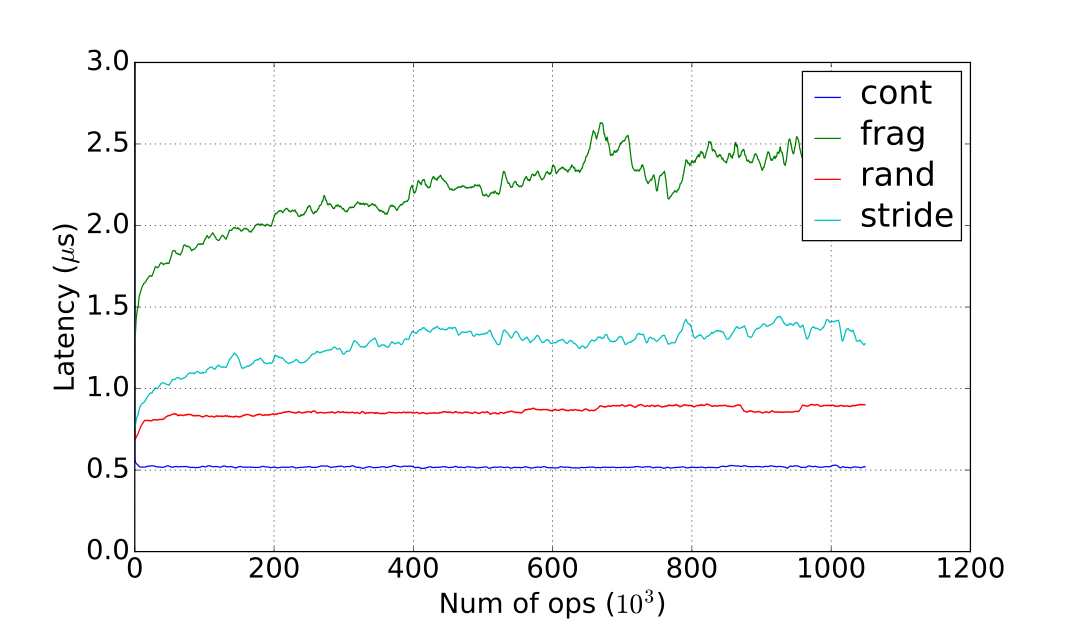
\includegraphics[width=\columnwidth]{figures/mmap_latency}
    \caption{Latency of memory operations}
    \label{fig:mmap_latency}
\end{figure}

\subsubsection{Memory}
Figure \ref{fig:mmap_mem_usage} shows the growth in memory usage of the system
for the workloads described in section \ref{ss_vm_area_struct}. The
\texttt{cont} workload coincides with the \texttt{control} workload as only the
first \texttt{mmap} operation allocates a \texttt{vm\_area\_struct}. The subsequent
operations are subsumed by the initial \texttt{vm\_area\_struct} as the mapped
regions are adjacent, and hence the memory usage does not increase despite the
large number of \texttt{mmap} operations.  The \texttt{stride} workload allocates a
\texttt{vm\_area\_struct} for each operation due to the separation of
allocations in the virtual address space. As a result, the memory usage
increases significantly as more memory is consumed with each \texttt{mmap} operation.
This is also the case for the \texttt{rand} workload which breaks up a single
\texttt{vm\_area\_struct} for a large area in the virtual address space into
multiple smaller areas, which results in the  allocation of a new structure for
every resize operation. The \texttt{rand} workload initially creates a new
\texttt{vm\_area\_struct} struct for each \texttt{mmap} operation. Eventually, these
allocations form larger contiguous allocations when two or more regions are
mapped next to each other, resulting in a single \texttt{vm\_area\_struct} being
used for that range. As a result, the memory usage begins to flatten out and
even decreases slightly as multiple \texttt{vm\_area\_struct}s are collapsed to
single structures. This is made clear by Figure \ref{fig:vm_area_struct_count}
which shows the growth \texttt{vm\_area\_struct} counts for each workload.
\begin{figure}
    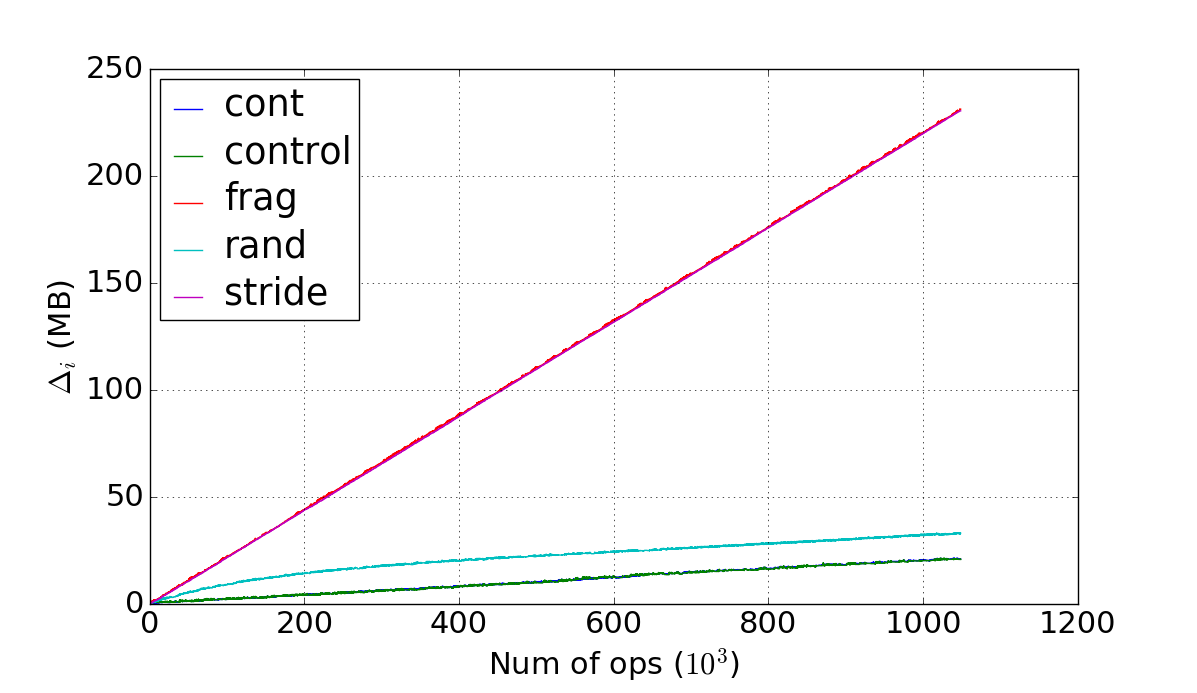
\includegraphics[width=\columnwidth]{figures/mmap_mem_usage}
    \caption{$\Delta_i$ adjusted with control for benchmarks}
    \label{fig:mmap_mem_usage}
\end{figure}

\begin{figure}
    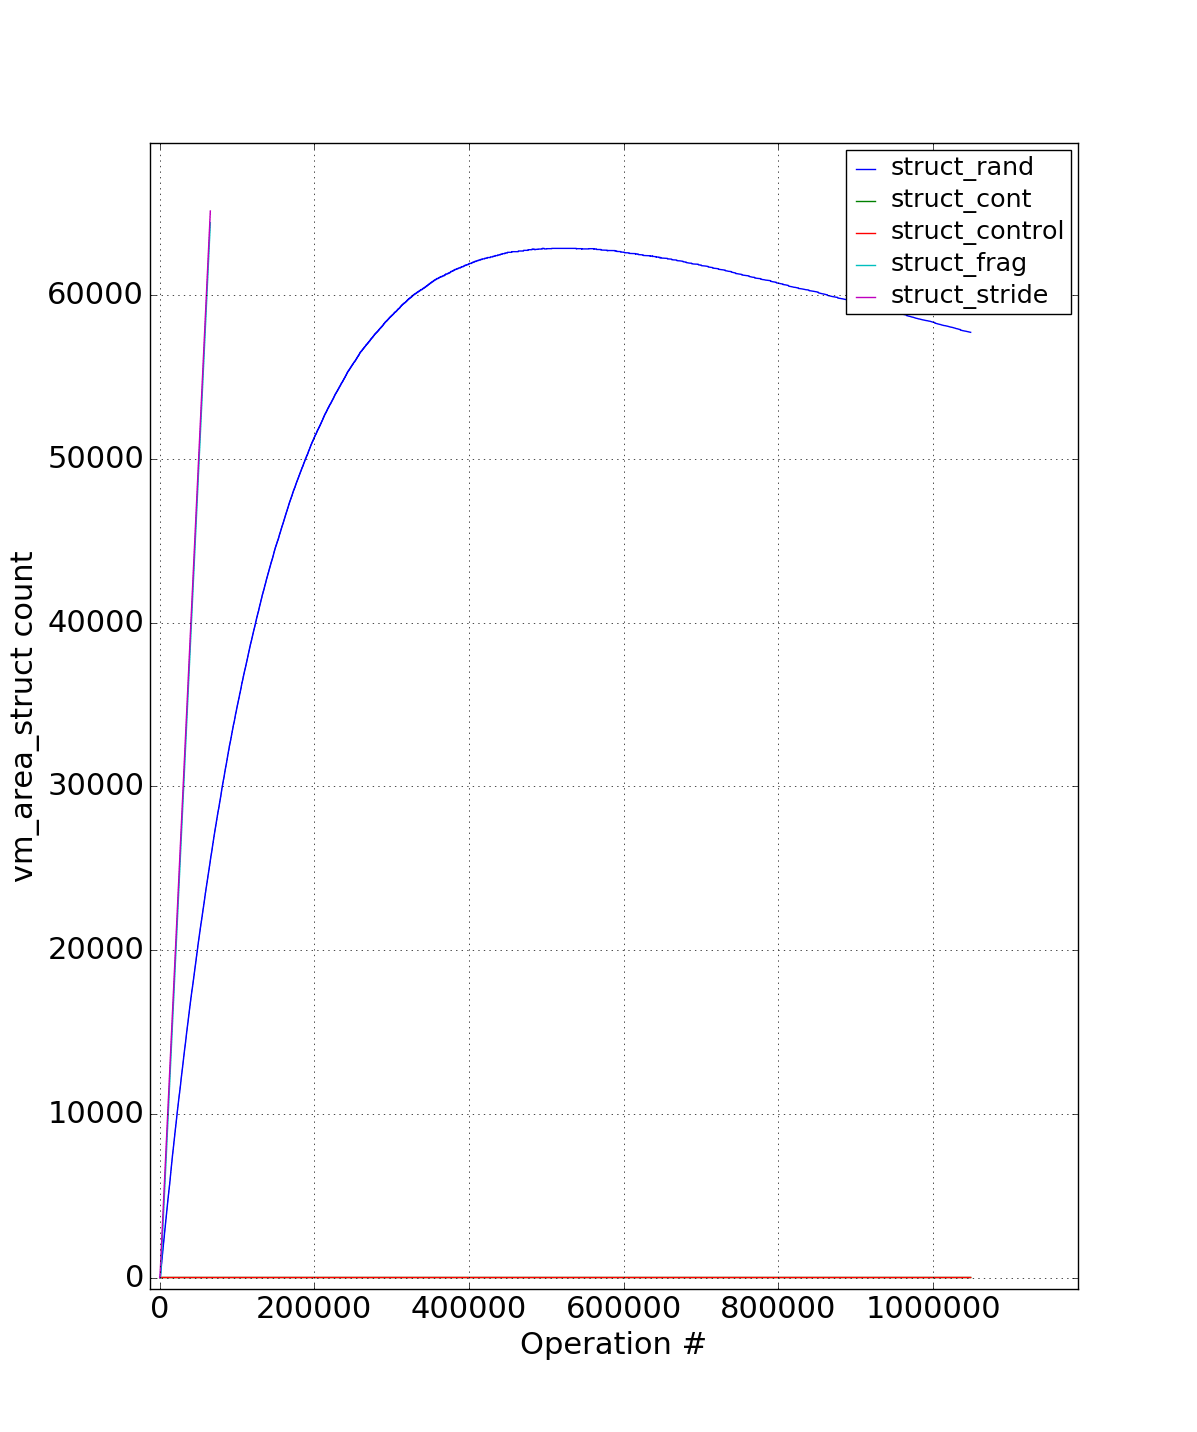
\includegraphics[width=\columnwidth]{figures/vm_area_struct_count}
    \caption{Number of \texttt{vm\_area\_struct}s for benchmarks}
    \label{fig:vm_area_struct_count}
\end{figure}


\subsection{Swapping Experiments}

\subsubsection{Memory}
Figure \ref{fig:swap_rss} shows the Resident Set Size of the system for the
experiments described in section \ref{swapping_memory_overhead}. The
\texttt{cont} workloads write to  adjacent 4KB pages in the address space. A
huge page of size 2MB is allocated (TODO: Is it 2MB?) when a new page is touched
initially. Subsequent 4KB pages that are touched are subpages of the 2MB page
allocated initially. As a result, the memory used by the workload is almost
equal to the amount of memory it has written to. The RSS thus increases linearly
until the system begins to swap when the number of free pages falls below a
threshold. The \texttt{rand} workload on the other hand writes to pages that are
not adjacent, and likely not subpages of a single huge page. As a result, a huge
page is allocated with almost every write, and the system starts to exhaust its
memory and begins swapping very quickly. Memory made available by kswapd is
quickly consumed by further writes and hence the memory used by the workload
continues to stay close to its peak value. As expected, the behavior is the same
irrespective of the size of the swap file.

\begin{figure}
    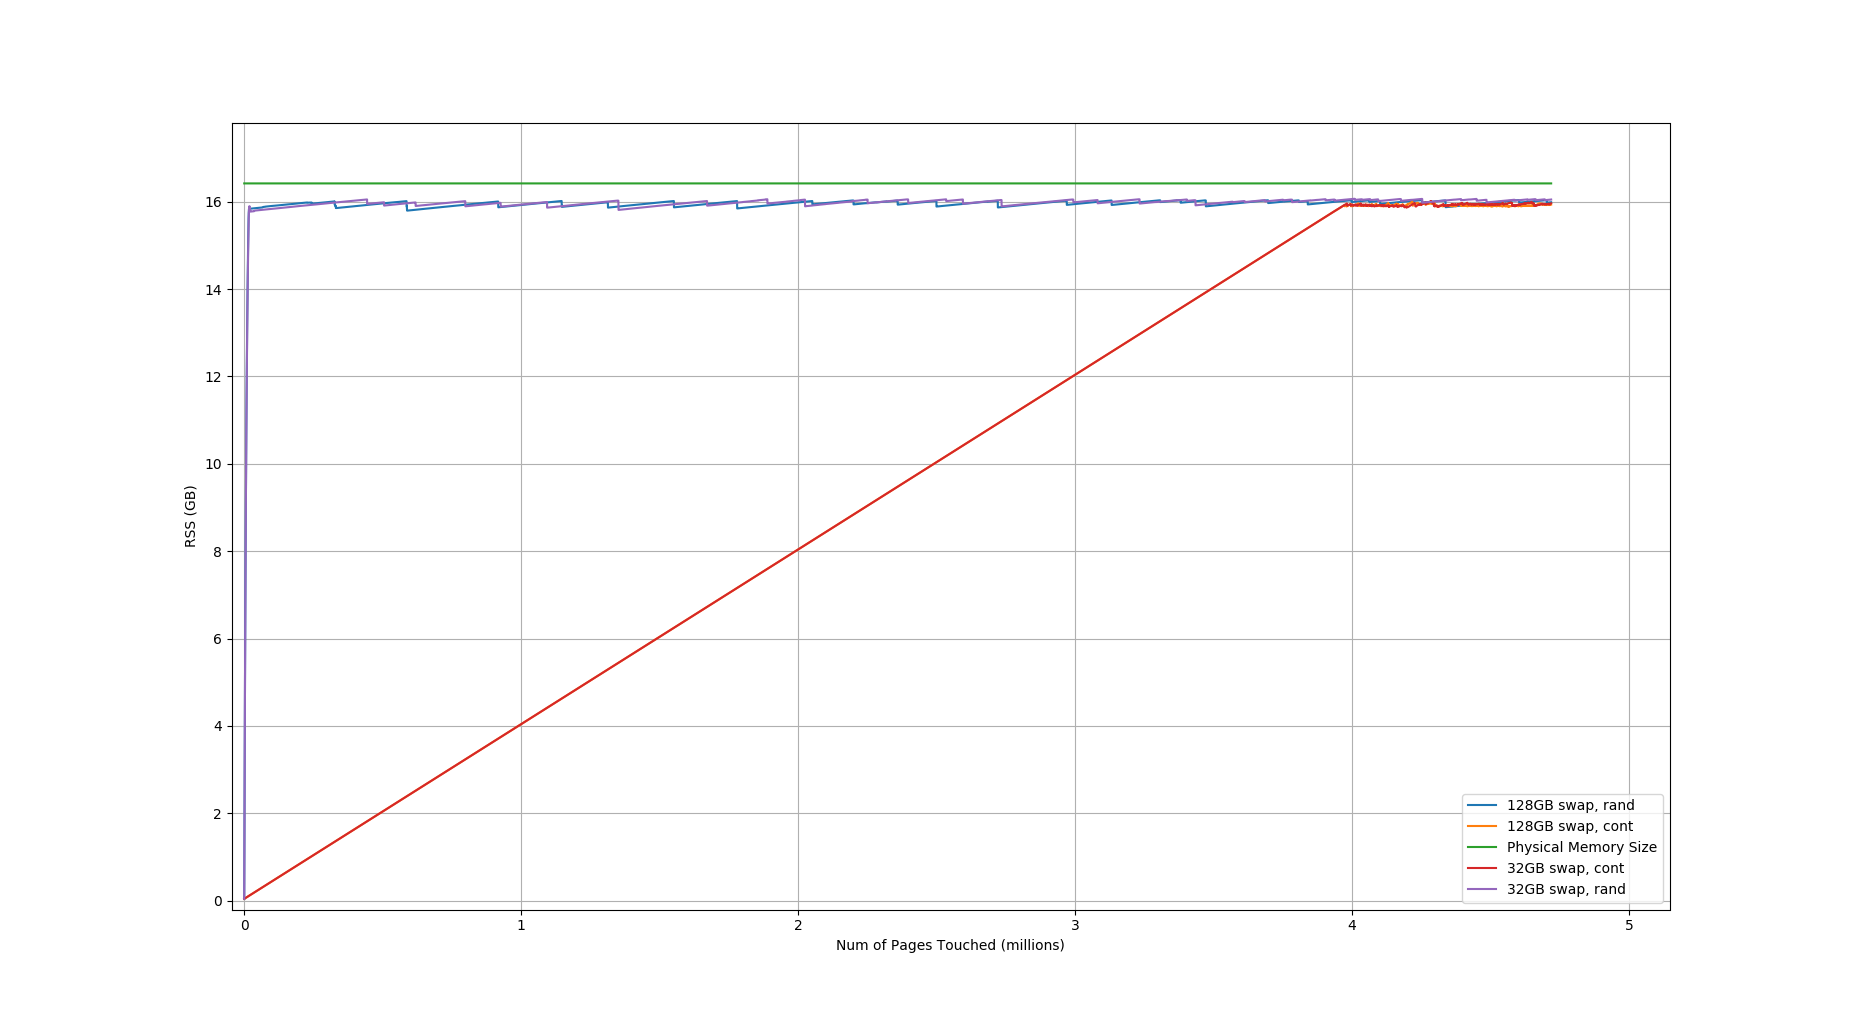
\includegraphics[width=\columnwidth]{figures/swap_rss}
    \caption{RSS while touching pages while swapping for random benchmark.}
    \label{swap_rss}
\end{figure}

\subsubsection{Time}

\begin{figure}
    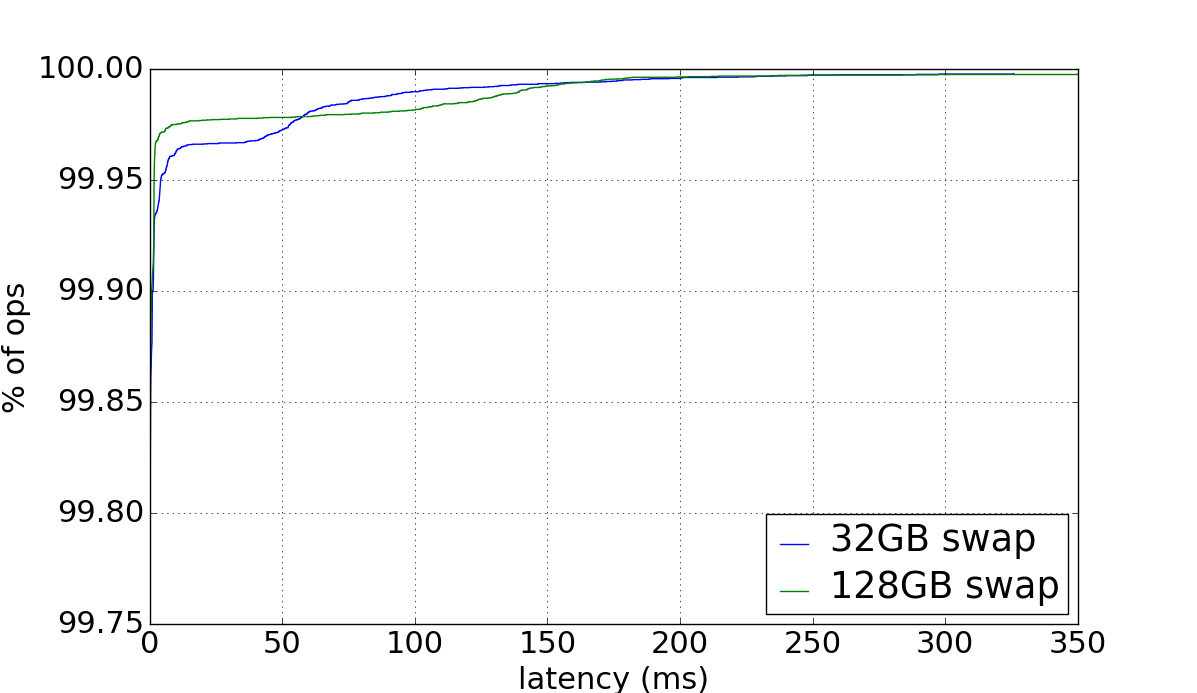
\includegraphics[width=\columnwidth]{figures/swap_touch_time_cont_cdf}
    \caption{CDF of time to touch a page while swapping for continuous
    benchmark. Notice that the y-axis scale is from 99.75\% to 100\%.
    \label{fig:swap_time_cont_cdf}}
\end{figure}

\begin{figure}
    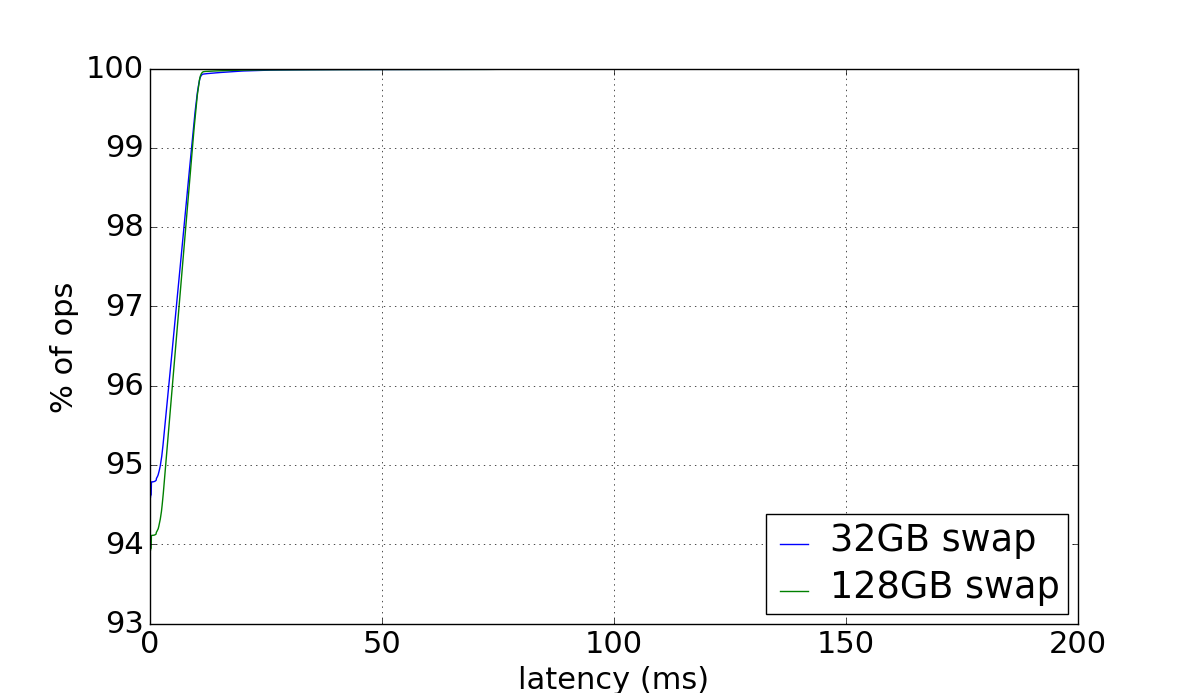
\includegraphics[width=\columnwidth]{figures/swap_touch_time_rand_cdf}
    \caption{CDF of time to touch a page while swapping for random benchmark.
    Notice that the y-axis scale is from 93\% to 100\%.\label{fig:swap_time_rand_cdf}}
\end{figure}

\begin{figure}
    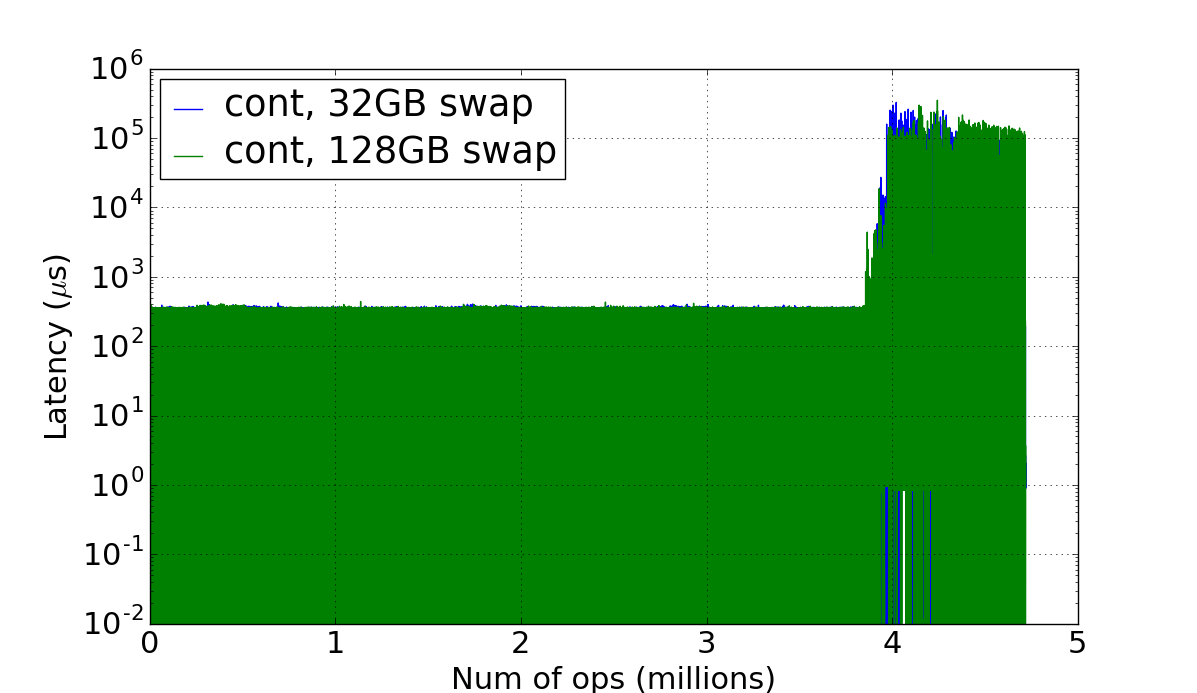
\includegraphics[width=\columnwidth]{figures/swap_time_cont}
    \caption{Time to touch a page while swapping for continuous benchmark.
    Notice that the y-scale is logarithmic.\label{fig:swap_time_cont}}
\end{figure}

\begin{figure}
    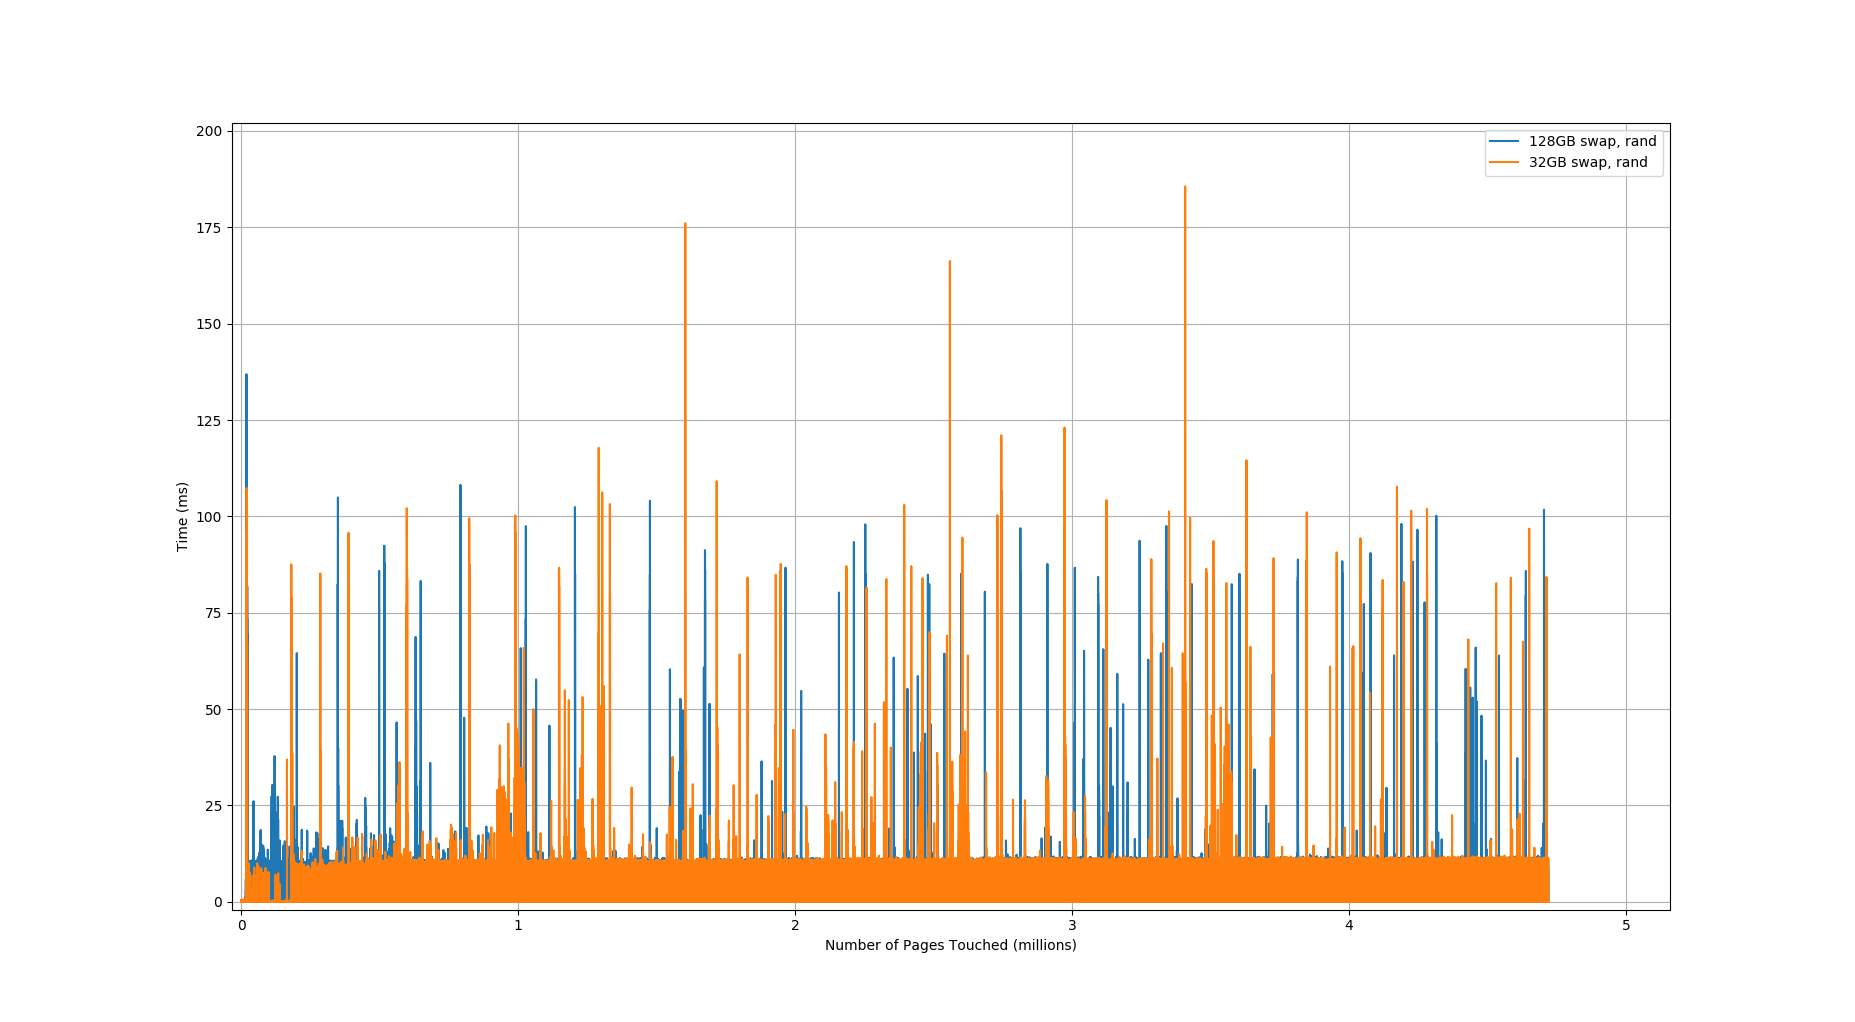
\includegraphics[width=\columnwidth]{figures/swap_time_rand}
    \caption{Time to touch a page while swapping for random
    benchmark.\label{fig:swap_time_rand}}
\end{figure}

\begin{figure}
    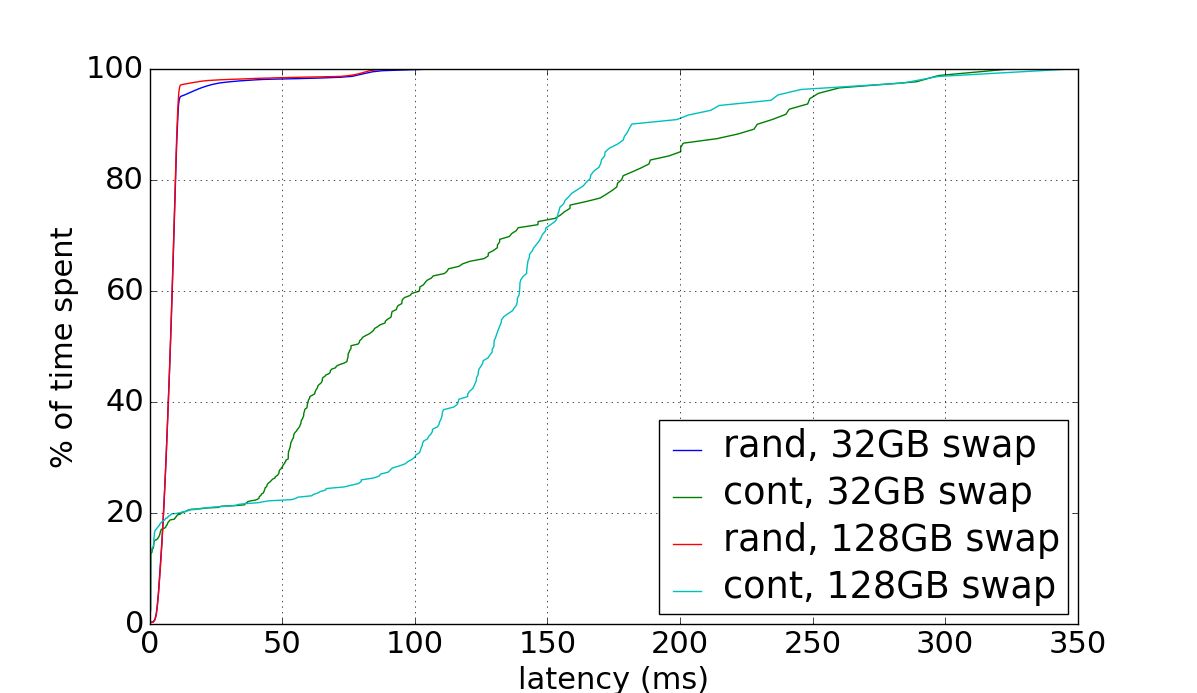
\includegraphics[width=\columnwidth]{figures/swap_time_cdf}
    \caption{CDF of amount of time spent on operations with a given
    latency.\label{fig:swap_time_cdf}}
\end{figure}

This experiment is designed to measure the impact of swapping on memory
operation latency. Figure \ref{fig:swap_time_cont} and Figure
\ref{fig:swap_time_rand} show the results.

The overall behavior is as expected. In the random benchmark, as before, all
memory is exhausted quickly, and the benchmark induces swapping soon after the
benchmark begins. Many memory accesses thus take milliseconds to complete
because they require paging in or out, which in turn depends on disk latency.
Even so, the majority of benchmark run time comes from a minority of accesses.
Figure \ref{fig:swap_time_rand_cdf} shows that as much as 95\% of memory
accesses occur on the micro-second scale. Of the remaining 5\%, almost all
accesses complete in less than 20ms. Moreover, notice that the size of the
swapfile makes very little difference in this workload because the disk has to
do random seeks regardless of swapfile size.

The continuous benchmark has more surprising results. Notice that Figure
\ref{fig:swap_time_cont} has a logarithmic y-scale. The system only begins to
swap after about 4M operations, as before. Unlike the random benchmark, we see a
number of operations that take hundreds of milliseconds. Figure
\ref{fig:swap_time_cont_cdf} shows that these only form a fraction of a percent
of all accesses done after swapping starts. However, Figure
\ref{fig:swap_time_cdf} shows that these few accesses form a majority of run
time; they impact performance significantly. (TODO: why do they happen?).

We also find that in the continuous benchmark, a larger swapfile actually has
slight more of these slow memory accesses. We believe this has to do with the
fact that the large swapfile has less disk locality, and so causes more disk
seeks when paging out. Figure \ref{fig:swap_time_cdf} shows that with a larger
swapfile, the continuous benchmark has a significantly higher number of
high-latency accesses as compared with the smaller swapfile.

~\\ \textbf{Conclusions} 

Large swapfiles should be created with disk locality or on SSDs.

Looking at 99.99-th percentile latencies is important because they can have a
lot of impact on overall run time.

TODO: what else?

\subsection{kswapd}

TODO: time: MARKM

TODO: khugepaged?


\section{Related Work}

The emergence of new technology has in the past often required operating systems
to change. Traditionally, OS researchers and developers benchmark and test their
solutions in new environments to demonstrate their efficacy before using them in
real systems. However, researchers do not always have access to new technology
for practical reasons; for example, large memory systems are still too expensive
for most research budgets. This is not the first time that researchers have been
forced to study systems in environments they do not have access to. This section
examines past approaches to studying these systems and motivates the need for
our work.

The emergence of the internet required businesses to buy expensive machines to
keep up with demand for their services, but systems researchers did not have
access to these machines. Alameldeen et al. describe how they simulate a
multi-million dollar server using a \$2000 workstation. To do this, they go
through several rounds of scaling down, optimizing, changing, and tuning both
the benchmarks and systems they test. For example, they scale down a workload to
fit in the 1GB memory of the machine they use and increase the number of threads
to improve parallelism \cite{2kmachine}. This methodology may be accurate, but
it requires modifying the benchmarks, which is error prone and time consuming;
it can be extremely difficult to validate changes to a benchmark. Ideally,
researchers can run large experimental workloads without changes, but the overheads
of current memory management systems prevent this from being practical.

Likewise, the Quartz emulator studies the behaviour of applications on
Non-volatile Memory (NVM) while actually running on top of DRAM. It uses
existing hardware capabilities to emulate the higher latency and lower bandwidth
of most NVM technologies. While Quartz does not address the fact that the actual
memory available to the applications on NVM might be orders of magnitude higher
than on DRAM, it demonstrates that new technologies may be emulated using
existing technology \cite{quartz}. (TODO: is this system still relavent?)

The Simics simulator uses demand paging for simulated environments, which means
that memory is only allocated when it is used. As long as the working set of
the target system fits in the host memory, performance will be tolerable.
However, in our work, we wish to study OS behavior under workloads that
actually use all available memory. Thus, the usefulness of demand paging is
greatly reduced because swapping causes disk latency to become the main
performance bottleneck. Moreover, the performance overhead of simulators like
Simics tends to be impractical because system state needs to be maintained by
the simulator \cite{simics}. We do not explore simulation further because it
can be orders of magnitude slower than native execution, making it infeasible
for studying large workloads or systems \cite{2kmachine}. However, the Simics
simulator illustrates the usefulness of memory management techniques such as
demand paging and the potential overheads of swapping.

A similar problem was encountered by researchers studying both large storage
drives and large distributed storage systems. David is a system that allows
storage and big data researchers to run large benchmarks requiring terabytes of
storage using off the shelf storage devices (which at that time were too small).
David creates a compressed version of the file system by physically storing only
metadata and discarding the contents of files. Reads to the disk causes David to
generate data on the fly. This decision choice is based on the observation that
most benchmarking frameworks do not care about the actual content of the files,
and that most of the storage capacity of a drive tends to be data rather than
metadata \cite{david}. The Exalt system uses a similar methodology for
large-scale distributed storage systems \cite{exalt}. This methodology provides
a promising direction for large-memory system studies. One may consider ignoring
the contents of a process’s heap and only storing kernel data structures and a
process’s code and stack segments. However, generating heap contents on the fly
is more difficult than generating disk contents because of the common use of
custom data structures. Moreover, on Linux, the kernel data structures for 1TB
of memory may also exceed the size of physical memory on current systems
\cite{simics}.

A virtualized environment can be used to provide a guest system with more memory
than is physically available to the host. A study of the limits of the KVM
hypervisor found that there is no fundamental limit to the size of guest
physical memory other than the hardware address width. However, currently, a
Linux host running KVM will require the guest memory to be backed by host
physical memory or host swap space \cite{ibmkvm}.  This means that when the
virtual machine uses the whole amount of memory allocated to it, the host can
swap pages to disk. The resulting poor performance can cause inaccurate
performance measurements when running benchmarks. It can also make large
benchmarks impractical.

Interestingly, many of non-volatile memory technologies are making their ways
into storage drives, such as Intel's recently-announced Optane SSDs. One
potential use of fast storage devices is for fast swapping space. Some
literature has proposed that small amounts of DRAM backed by large amounts of
fast swap space can be a scalable alternative to having large amounts of fast
RAM (TODO: cite). (TODO: can we have this in our report?). In such a system,
the overhead of swapping may become a bottleneck.

Prefetching pages from swap space can offer a way to mitigate the overhead of
memory overcommitment, possibly making large virtual machines a viable
mechanism for studying large memory systems. When there is significant memory
pressure, even pages which are likely to be accessed soon are swapped out to
disk. They are faulted back into memory when accessed, resulting in significant
performance cost.  Charm++ uses a programming model where computations can be
scheduled by the language runtime. A designated thread can prefetch pages
required by a computation, averting page faults \cite{charmpp}. Rather than
implement page prefetching in a language runtime, one might implement a
prefetcher in the swapping subsystem, making it general purpose. A large body
of work already exists on hardware prefetching for processor caches, on which a
swap prefetcher might draw for inspiration (TODO: cite). However, this approach
can only work if page access patterns are predictable. Moreover, the high
latency of disks implies that prefetchers would have to predict the very
distant future (e.g. seconds ahead of execution). (TODO: Mike's comment on the
previous version of this paragraph said that it was ``too distant/off topic''.
Is it better now? I feel like prefetching was an idea that we considered too
much to leave out...)

Gupta et al. built an emulator for high speed networks using a technique called
time dilation, which slows down the OS clock to make it appear that external
events are occurring faster. This allows the system to emulate network links
with speeds that are currently not available. The implementation is based on
the VMs and Xen hypervisor; Xen delivers the timer interrupts to the guest at a
lower rate than hardware hence  slowing down the guest’s clock \cite{timedil}.
A similar approach may be applied for large memory system studies to slow down
guest time while paging in and out large portions of memory. This will allows
the system to believe that it is reading data from the memory while actually
most of that data is being read from the disk.

Finally, there have been studies which look at the performance overheads
associated with current implementations of virtual memory and suggest mechanisms
to mitigate them. RadixVM tries to overcome performance issues in highly
concurrent workloads due to serialization of memory management operations on
kernel data structures \cite{radixvm}. This work demonstrates that many parts of
existing memory management schemes are not scalable to larger systems.
Similarly, in our work, we wish to examine scalability limitations of memory
management in the Linux kernel. Other studies have suggested that \texttt{struct
page}, \texttt{struct vm\_area\_struct}, and page tables tend to comprise a
large portion of memory management overhead \cite{simics} (TODO: cite the LWN
paper).

\bibliography{references}{}
\bibliographystyle{plain}

\end{document}
